\documentclass{article}
\usepackage{../../settings}

\begin{document}
\hexcover{Py 心寫程式}{學習歷程}{作者:曾嘉禾}{Dandelion}{電算社}

\begin{large}
\begin{boxpar}{Dandelion}{說明}
利用 Python 寫出像樣的遊戲
\end{boxpar}
\begin{boxpar}{Dandelion}{動機}
雖然我有在寫程式,但常常好奇在那個黑盒子外還可以用程式寫出其他很酷的應用,很經典的例子就是遊戲。一直以來,我更是好奇程式是如何處理視窗、按鈕、元件等等的圖形化介面的項目。來到師大附中博覽會,看到電算社能夠利用python
的 pygame
做成各式各樣好玩遊戲的樣子尤其感到羨慕。所以這次為了圓夢以及完成擔任電算社靜態展的義務,決定與組員以
pygame 寫出像樣的遊戲,花點心思懷抱與追求自己的夢想。
\end{boxpar}
    \begin{boxpar}{Dandelion}{學習過程}
        在學習 pygame 的剛開始,接觸到的最基本的 pygame 程式碼後驚訝的發現竟然有 while true:
        的危險程式,但後來才知道只要讓程式碼有條件地退出就不會產生太多問題,所以在寫
        pygame 程式時小心一點就不用擔心。
        \begin{mintbox}{範例程式碼}{Dandelion}{python}
# Example file showing a basic pygame "game loop"
import pygame

# pygame setup
pygame.init()
screen = pygame.display.set_mode((1280, 720))
clock = pygame.time.Clock()
running = True

while running:
    # poll for events
    # pygame.QUIT event means the user clicked X to close your window
    for event in pygame.event.get():
        if event.type == pygame.QUIT:
            running = False

    # fill the screen with a color to wipe away anything from last frame
    screen.fill("purple")

    # RENDER YOUR GAME HERE

    # flip() the display to put your work on screen
    pygame.display.flip()

    clock.tick(60)  # limits FPS to 60

pygame.quit()
        \end{mintbox}
    \end{boxpar}

    \newpage
\begin{boxpar}{Dandelion}{遇到的問題:不清楚 pygame.display}
一開始常常遇到的問題就是 pyagme.display 的管理。因為 GUI
    遊戲需要處理圖形並顯示在畫面上,所以管理顯示器的 pygame.display
    就相當重要。不過身為初學者常常因為不熟悉 pygame.display
    的運作方式而常常導致圖形在顯示器上錯位。
    \begin{boxpar}{Dandelion}{解決方式}
        查詢 Documentation 是最簡單的解決方式。身為未來想當程式設計師的我,必須要學習如何閱讀
        Documentation。因為有時在問別人問題或放棄之前,其實已經有人在網路上早就解答過了。當時我有去
        \href{https://www.pygame.org/docs/ref/display.html}{pygame 官網} 查詢,更是去
        \href{https://www.youtube.com/watch?v=C8YtdC8mxTU}{YouTube 上}
        查詢影片。在種種的查詢下,我也逐漸得知 framerate fps
        或是其他視窗管理功能的對應 pygame
        程式碼。完全熟悉他們後,我對我自己所下的功夫感到大有成就感。
    \end{boxpar}
\end{boxpar}
\begin{boxpar}{Dandelion}{遇到的問題:組員之間無法溝通}
    身為一位電算社靜態展學術長,組員之間的溝通以及進度分配是十分重要的。一開始,因為溝通不足而導致自己誤會組員耍賴不做事。但經過一次次的線上討論與會議以及釐清每位組員的個別需求後發現其實組員是肯認真工作的。最後發現我與組員逐漸的打成一片,是一件極為幸福的事情。
\end{boxpar}
\begin{boxpar}{Dandelion}{成品}
    我把原始碼\href{https://github.com/hsnucrc46/crcproject}{commit 到 GitHub
    上}並且以 GPLv3 的 copyleft 授權書授權。
    圖片
    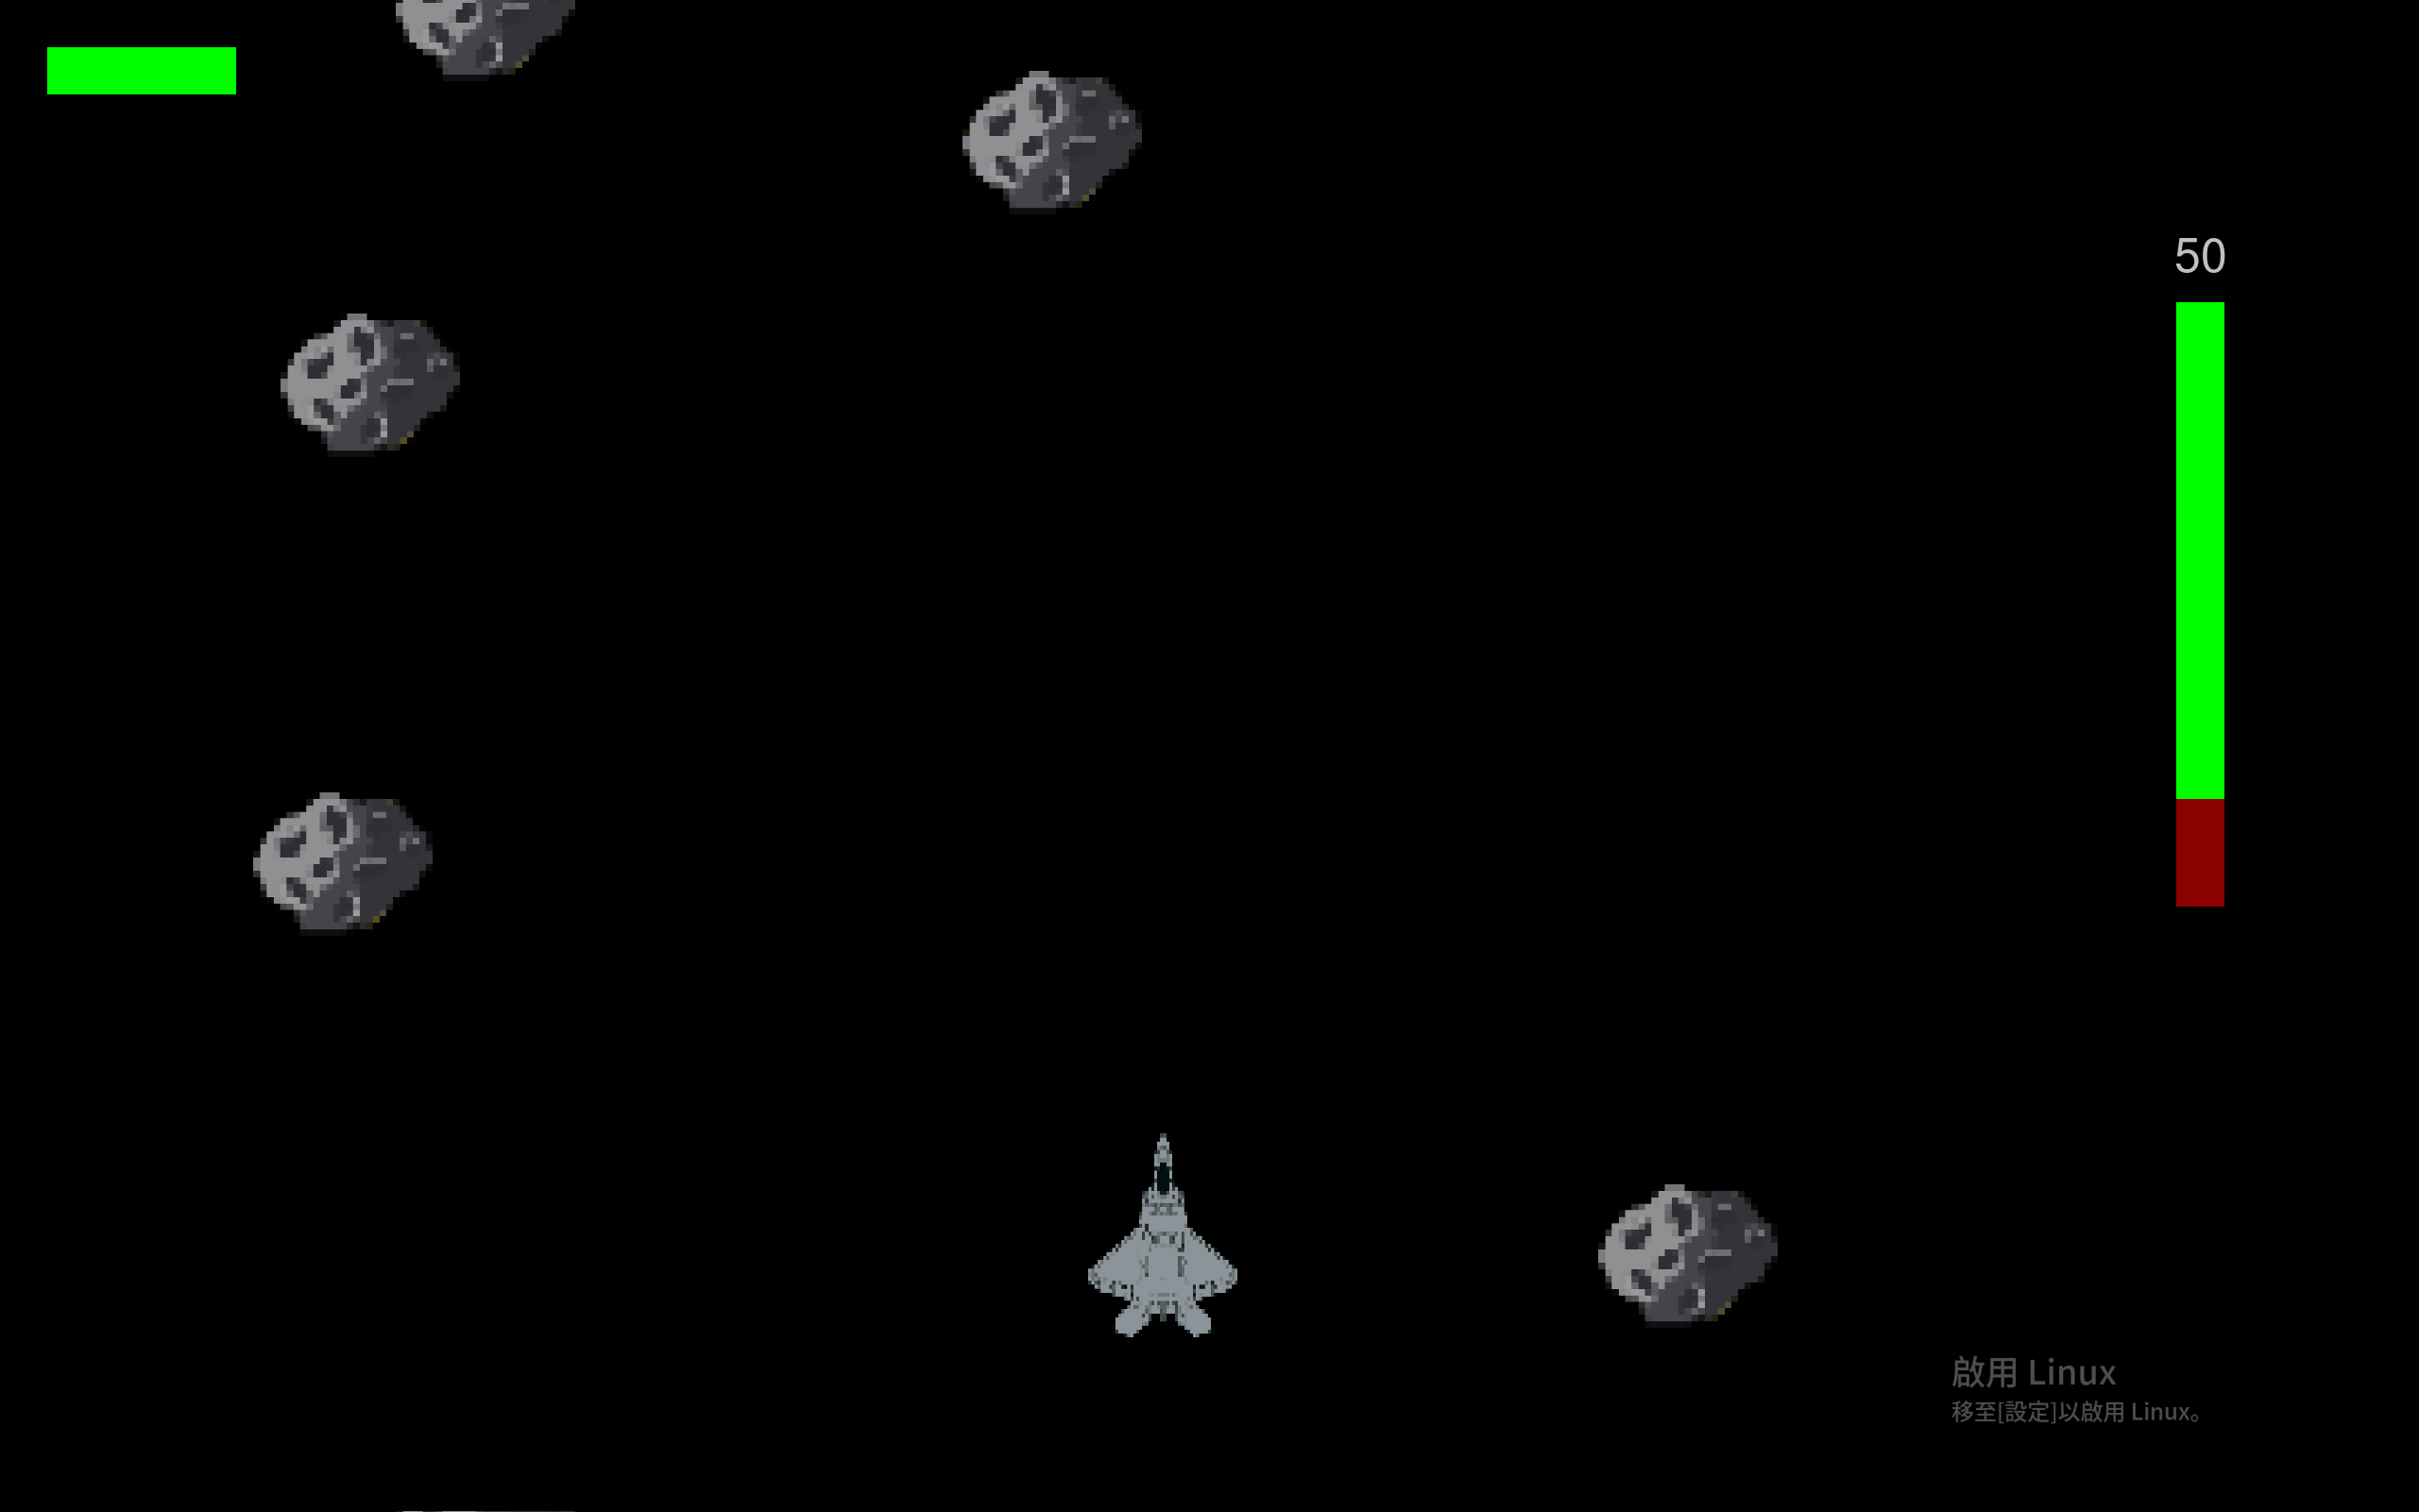
\includegraphics[width=\linewidth]{src/game.png}
\end{boxpar}
\begin{boxpar}{Dandelion}{結尾}
    在這次的自主學習,我發現寫程式一直以來不是一個人的事,是大家的事。自行找答案更是一位程式設計師必須具備的基本能力。所以未來如果我有參與其他活動也會盡力的與組員有良好的溝通並且在麻煩別人之前自己找尋答案以更有效率的完成大家最後的共同目標。
\end{boxpar}
\end{large}
\end{document}
